\documentclass[sigconf,nonacm]{acmart}

\usepackage{tikz}
\usetikzlibrary{shapes.geometric,arrows.meta,positioning,matrix}

\AtBeginDocument{%
  \providecommand\BibTeX{{Bib\TeX}}}

\acmConference[INF1824]{Projeto Orientado IV -- INF1824}{2026}{Rio de Janeiro, RJ, Brasil}
\acmBooktitle{Relatório Técnico -- Projeto Orientado IV (INF1824), PUC-Rio}

\begin{document}

\title{Identificação e Correção de Gargalos de Level Design via Aprendizado por Reforço Profundo}

\author{Robert Ronald Calla Maguiña}
\affiliation{%
  \institution{Departamento de Informática, PUC-Rio}
  \city{Rio de Janeiro}
  \state{RJ}
  \country{Brasil}}
%% Descomente e preencha com seu e-mail institucional, se desejar exibi-lo:
%% \email{seu-email@aluno.puc-rio.br}

\renewcommand{\shortauthors}{Calla Maguiña}

\begin{abstract}
Este trabalho relata o andamento do desenvolvimento de um sistema de
Inteligência Artificial voltado à identificação e correção automática de
gargalos de \emph{level design} em fases 2D baseadas em física. O ambiente de
desenvolvimento é estruturado na engine Godot 4.7, com foco no processamento
de mecânicas multiplayer. Diferentemente de abordagens tradicionais de
navegação (\emph{pathfinding}), o objetivo é treinar um agente capaz de
analisar a topologia do mapa, identificar zonas de estrangulamento que
prejudicam a fluidez do jogo e aplicar técnicas de geração de conteúdo para
sugerir adaptações no cenário. Propomos uma arquitetura que combina a
extração estruturada do ambiente em uma matriz 2D, o processamento espacial
por meio de Redes Neurais Convolucionais (CNN) e um agente de Aprendizado por
Reforço Profundo (DRL) inspirado em conceitos de \emph{Curiosity-Driven
Exploration} e de \emph{Procedural Content Generation via Reinforcement
Learning} (PCGRL). Formalizamos o problema como um Processo de Decisão de
Markov, detalhamos as decisões de projeto para cada componente do pipeline
(representação de estado, extrator convolucional, política e função de
recompensa híbrida intrínseca/extrínseca), descrevemos o estado atual da
implementação e propomos uma metodologia de avaliação -- com métricas,
baselines e protocolo experimental -- para os próximos ciclos do projeto.
Discutimos ainda as limitações e os riscos de \emph{reward hacking}
inerentes à abordagem, bem como um roteiro de trabalhos futuros.
\end{abstract}

\keywords{Level Design, Aprendizado por Reforço Profundo, Geração
  Procedural de Conteúdo, Curiosity-Driven Exploration, Godot Engine,
  Playtesting Automatizado, Redes Neurais Convolucionais}

\maketitle

\section{Introdução}

O \emph{level design} é um dos pilares da experiência de jogo: a forma como
corredores, salas, obstáculos e rotas alternativas são dispostos determina
diretamente o ritmo, a dificuldade percebida e a fluidez com que o jogador
avança pela fase. Contudo, identificar manualmente pontos de fricção que
prejudicam essa fluidez -- os chamados \emph{gargalos} (\emph{bottlenecks})
-- é um processo custoso, subjetivo e dependente de extensas sessões de
\emph{playtesting} humano. Em produções com ciclos de iteração curtos, ou em
fases geradas proceduralmente, esse custo se torna ainda mais crítico, pois
cada nova versão do nível exigiria uma nova rodada de testes manuais.

Este trabalho relata o progresso da pesquisa e desenvolvimento de uma
aplicação de Inteligência Artificial para identificação e correção desses
gargalos. O ambiente de desenvolvimento está sendo estruturado na engine
Godot 4.7~\cite{godotengine}, com foco no processamento de fases 2D baseadas
em física e mecânicas multiplayer, um domínio no qual gargalos de
navegação afetam não apenas um jogador isolado, mas a dinâmica de disputa
por espaço entre múltiplos agentes.

\subsection{Motivação}

A motivação central do projeto é que ferramentas automáticas de
\emph{playtesting} baseadas em IA podem reduzir o custo de iteração do
processo de \emph{level design}, permitindo que designers recebam
retroalimentação quantitativa sobre a qualidade estrutural de um nível antes
mesmo de exposê-lo a testadores humanos. Diferente de heurísticas estáticas
de análise de grafos (por exemplo, medidas de centralidade sobre o grafo de
navegabilidade), um agente treinado por reforço pode capturar efeitos
dinâmicos do \emph{gameplay} -- como congestionamento causado por múltiplos
jogadores disputando o mesmo corredor -- que não são triviais de expressar
como regra fixa.

\subsection{Definição do Problema}

O objetivo do projeto é ir além da simples navegação (\emph{pathfinding}).
A meta é treinar um agente de aprendizado de máquina capaz de:
\begin{enumerate}
  \item analisar a topologia do mapa a partir de uma representação
    estruturada e independente de renderização gráfica;
  \item identificar zonas de estrangulamento que prejudicam a fluidez do
    jogo, isto é, regiões do mapa em que o fluxo de travessia entre pontos
    de interesse é anormalmente baixo; e
  \item aplicar técnicas de geração de conteúdo para sugerir adaptações no
    cenário que aliviem esses gargalos, fechando o ciclo entre diagnóstico
    e correção.
\end{enumerate}
Em outras palavras, o agente não deve apenas percorrer o nível, mas
aprender a apontar -- e eventualmente corrigir -- falhas estruturais de
\emph{design}.

\subsection{Contribuições}

As contribuições deste relatório de andamento são:
\begin{itemize}
  \item uma arquitetura de representação de ambiente independente de
    renderização gráfica, baseada em matrizes 2D extraídas diretamente do
    \texttt{TileMap} e do \texttt{NavigationServer2D} do Godot;
  \item uma formalização do problema como um Processo de Decisão de Markov
    (MDP), com espaço de estados, espaço de ações e uma proposta de função
    de recompensa híbrida (intrínseca + extrínseca);
  \item uma proposta de pipeline \emph{CNN~+~DRL} para transformar essa
    representação em decisões de ação sobre o nível, incluindo a escolha
    justificada do algoritmo de otimização de política e do módulo de
    curiosidade;
  \item uma metodologia de avaliação planejada, com métricas, baselines e
    protocolo experimental, ainda a ser executada nos próximos ciclos do
    projeto; e
  \item uma discussão inicial sobre limitações e riscos metodológicos,
    notadamente o risco de \emph{reward hacking}.
\end{itemize}

\subsection{Organização do Documento}

O restante deste artigo está organizado da seguinte forma. A
Seção~\ref{sec:relacionados} discute trabalhos relacionados em geração
procedural de conteúdo via aprendizado por reforço, \emph{playtesting}
automatizado e exploração guiada por curiosidade. A
Seção~\ref{sec:formalizacao} formaliza o problema como um MDP. A
Seção~\ref{sec:arquitetura} detalha a arquitetura do sistema proposto. A
Seção~\ref{sec:estado} descreve o estado atual da implementação. A
Seção~\ref{sec:avaliacao} propõe a metodologia de avaliação. A
Seção~\ref{sec:discussao} discute limitações e riscos. A
Seção~\ref{sec:etica} discute considerações éticas e de uso responsável. A
Seção~\ref{sec:futuro} apresenta o roteiro de trabalhos futuros, e a
Seção~\ref{sec:conclusao} conclui o artigo.

\section{Trabalhos Relacionados}
\label{sec:relacionados}

O uso de aprendizado por reforço para geração e avaliação de conteúdo de
jogos vem se consolidando como uma alternativa aos métodos tradicionais de
geração procedural baseados em regras ou busca (\emph{search-based
PCG})~\cite{shaker2016procedural}. Esta seção revisa três frentes que
sustentam a arquitetura proposta: geração procedural via aprendizado por
reforço, \emph{playtesting} automatizado com agentes humanoides, e
exploração guiada por curiosidade.

\subsection{Geração Procedural de Conteúdo via Aprendizado por Reforço}

Khalifa et~al.~\cite{khalifa2020pcgrl} propõem o PCGRL (\emph{Procedural
Content Generation via Reinforcement Learning}), no qual a geração de
níveis é formulada como um problema sequencial de decisão: um agente edita
o mapa tile a tile e recebe recompensas conforme métricas de qualidade do
nível resultante (por exemplo, conectividade, número de inimigos alcançáveis
ou tamanho do caminho mais curto). Diferentemente de modelos generativos
treinados por aprendizado supervisionado sobre corpora de níveis existentes,
o PCGRL não depende de grandes conjuntos de dados anotados, e sim de uma
função de recompensa bem definida sobre o espaço de níveis -- uma
característica central que buscamos reaproveitar neste projeto. Essa
formulação inspira diretamente a representação de estado e o espaço de ação
discutidos na Seção~\ref{sec:arquitetura} deste trabalho.

\subsection{Playtesting Automatizado com Agentes Humanoides}

Na frente de \emph{playtesting} automatizado, De Woillemont
et~al.~\cite{dewoillemont2022automated} utilizam aprendizado por reforço
para gerar agentes com estilos de jogo semelhantes aos humanos, permitindo
testar um jogo sob perfis de comportamento variados sem depender de
testadores humanos para cada iteração. Essa linha de trabalho parte da
premissa de que um agente puramente ótimo (por exemplo, um agente que
sempre encontra o caminho mais curto) não é representativo do comportamento
real de jogadores, que exploram, hesitam e cometem erros. Sestini
et~al.~\cite{sestini2022automated} avançam essa linha propondo trajetórias
proximais condicionadas por curiosidade (\emph{curiosity-conditioned
proximal trajectories}) para validação automatizada de \emph{gameplay},
combinando exploração guiada por curiosidade com métodos de otimização de
política por região de confiança para detectar estados de jogo raros ou
problemáticos (por exemplo, situações de \emph{softlock} ou exploração de
\emph{bugs}).

\subsection{Exploração Guiada por Curiosidade}

O componente de exploração guiada por curiosidade utilizado neste projeto
segue a formulação do \emph{Intrinsic Curiosity Module} (ICM) proposta por
Pathak et~al.~\cite{pathak2017curiosity}, na qual um modelo preditivo
aprende a antecipar a representação latente do próximo estado a partir do
estado e da ação atuais; o erro dessa predição é utilizado como recompensa
intrínseca, incentivando o agente a visitar regiões do ambiente cuja
dinâmica ainda não foi bem modelada. Esse mecanismo é particularmente
adequado ao nosso cenário, pois gargalos de \emph{level design} tendem a
corresponder a regiões pouco visitadas por políticas ingênuas de navegação,
exatamente as regiões que um sinal de curiosidade tende a priorizar.

\subsection{Posicionamento deste Trabalho}

A Tabela~\ref{tab:relacionados} resume o posicionamento do presente
trabalho em relação aos três trabalhos discutidos. O projeto se posiciona
na interseção dessas linhas: assim como o PCGRL, utiliza uma representação
matricial do nível como estado de um processo de decisão de Markov; e,
assim como os trabalhos de \emph{playtesting} automatizado, incorpora
exploração orientada por curiosidade -- não para gerar estilos de jogador,
mas para que o próprio agente descubra e sinalize regiões do mapa com
baixo fluxo de travessia, tratando a detecção de gargalos como o objetivo
central da recompensa, e não apenas como um subproduto da exploração.

\begin{table}
  \caption{Posicionamento em relação aos trabalhos relacionados}
  \label{tab:relacionados}
  \begin{tabular}{p{0.24\linewidth}p{0.62\linewidth}}
    \toprule
    \textbf{Trabalho} & \textbf{Foco principal} \\
    \midrule
    PCGRL~\cite{khalifa2020pcgrl} & Geração de níveis tile a tile via RL,
      recompensa sobre métricas globais de qualidade do nível. \\
    De~Woillemont et~al.~\cite{dewoillemont2022automated} & Geração de
      agentes de \emph{playtesting} com estilos de jogo humanoides. \\
    Sestini et~al.~\cite{sestini2022automated} & Validação automatizada de
      \emph{gameplay} via exploração condicionada por curiosidade. \\
    \textbf{Este trabalho} & Diagnóstico e sinalização de gargalos de
      \emph{level design} como objetivo central da recompensa, combinando
      representação matricial (PCGRL) com curiosidade (ICM) para priorizar
      regiões de baixo fluxo. \\
    \bottomrule
  \end{tabular}
\end{table}

\section{Formalização do Problema}
\label{sec:formalizacao}

\subsection{Gargalos de Level Design}

Definimos informalmente um gargalo como uma região do nível cujo fluxo de
travessia -- o número de vezes que agentes passam por aquela região durante
um episódio de \emph{gameplay}, normalizado pelo tempo total do episódio --
é significativamente menor do que o esperado para uma região com
conectividade equivalente no grafo de navegação. Essa definição captura
tanto gargalos ``estruturais'' (um corredor estreito que fisicamente limita
a passagem simultânea de múltiplos jogadores) quanto gargalos
``comportamentais'' (uma bifurcação que jogadores tendem a evitar por
parecer, subjetivamente, menos vantajosa).

\subsection{Processo de Decisão de Markov}

Modelamos o problema como um Processo de Decisão de Markov (MDP)
$\langle \mathcal{S}, \mathcal{A}, P, R, \gamma \rangle$, no qual:

\begin{itemize}
  \item $\mathcal{S}$ é o espaço de estados, definido pela matriz 2D
    $G \in \{0,1\}^{H \times W}$ que representa o nível (Seção~\ref{sec:representacao}),
    possivelmente aumentada por canais adicionais que codificam a posição
    do agente e de pontos de interesse (entrada, saída, itens);
  \item $\mathcal{A}$ é o espaço de ações, detalhado na
    Seção~\ref{sec:acao};
  \item $P(s_{t+1} \mid s_t, a_t)$ é a dinâmica de transição, determinada
    pelo motor de física e navegação do Godot;
  \item $R(s_t, a_t, s_{t+1})$ é a função de recompensa, detalhada na
    Seção~\ref{sec:recompensa}; e
  \item $\gamma \in [0,1)$ é o fator de desconto.
\end{itemize}

O objetivo do treinamento é encontrar uma política $\pi_\theta(a_t \mid
s_t)$, parametrizada por uma rede neural com parâmetros $\theta$, que
maximize o retorno esperado
\begin{equation}
  J(\theta) = \mathbb{E}_{\pi_\theta}\!\left[ \sum_{t=0}^{T} \gamma^t
  R(s_t, a_t, s_{t+1}) \right].
  \label{eq:objective}
\end{equation}

\subsection{Espaço de Estados}
\label{sec:representacao}

O estado observado pelo agente em cada instante $t$ é a matriz $G_t$
descrita na Seção~\ref{sec:representacao-ambiente}, processada por um
extrator convolucional $\phi(\cdot)$ (Seção~\ref{sec:cnn}) que produz um
vetor de características latente $z_t = \phi(G_t) \in \mathbb{R}^d$. Esse
vetor latente é a entrada tanto da rede de política quanto do módulo de
curiosidade.

\subsection{Espaço de Ações}
\label{sec:acao}

Propomos um espaço de ações híbrido, refletindo a natureza em duas fases do
problema (navegação e, posteriormente, edição de conteúdo):
\begin{itemize}
  \item \textbf{Ações de navegação}: um vetor de deslocamento discreto
    $a^{\text{nav}} \in \{\text{norte}, \text{sul}, \text{leste},
    \text{oeste}, \text{parado}\}$, compatível com a granularidade da
    matriz de \emph{tiles};
  \item \textbf{Ações de sinalização/edição} (fase posterior do projeto):
    $a^{\text{edit}} \in \{\text{nenhuma}, \text{marcar gargalo},
    \text{remover bloqueio}, \text{adicionar bloqueio}\}$, aplicadas à
    célula da matriz correspondente à posição atual do agente.
\end{itemize}
Na fase atual do projeto, apenas $a^{\text{nav}}$ está em uso; o espaço de
edição será incorporado progressivamente, conforme discutido na
Seção~\ref{sec:futuro}.

\subsection{Função de Recompensa}
\label{sec:recompensa}

Propomos uma função de recompensa híbrida, combinando um termo extrínseco
$r^{\text{ext}}_t$, responsável por penalizar gargalos, e um termo
intrínseco $r^{\text{int}}_t$, responsável por guiar a exploração:
\begin{equation}
  R(s_t, a_t, s_{t+1}) = r^{\text{ext}}_t + \beta \, r^{\text{int}}_t,
  \label{eq:reward}
\end{equation}
em que $\beta$ é um coeficiente de balanceamento entre os dois termos.

O termo extrínseco penaliza células de baixo fluxo de travessia. Seja
$\tau(v)$ o fluxo acumulado de travessia da célula $v$ ao longo de uma
janela de $N$ episódios, e $\theta_\tau$ um limiar abaixo do qual uma célula
é considerada um gargalo. Definimos
\begin{equation}
  r^{\text{ext}}_t = -\sum_{v \,\in\, \mathcal{V}(s_t)} w(v) \cdot
    \mathbb{1}\!\left[\tau(v) < \theta_\tau\right],
  \label{eq:reward-ext}
\end{equation}
em que $\mathcal{V}(s_t)$ é a vizinhança imediata da posição do agente em
$s_t$ e $w(v)$ é um peso proporcional à centralidade da célula $v$ no grafo
de navegação -- de modo que gargalos em rotas centrais sejam penalizados mais
fortemente do que gargalos em regiões marginais do mapa.

O termo intrínseco segue a formulação do ICM~\cite{pathak2017curiosity}: um
modelo preditivo $f_\psi$ estima a representação latente do próximo estado,
$\hat{z}_{t+1} = f_\psi(z_t, a_t)$, e o erro de predição é utilizado como
recompensa,
\begin{equation}
  r^{\text{int}}_t = \frac{\eta}{2} \, \lVert \hat{z}_{t+1} - z_{t+1}
    \rVert_2^2,
  \label{eq:reward-int}
\end{equation}
em que $\eta$ é uma constante de escala. A intuição é que regiões do nível
cuja dinâmica é mal modelada pelo agente -- tipicamente regiões pouco
visitadas, como gargalos -- geram maior erro de predição e, portanto, maior
recompensa intrínseca, complementando o sinal extrínseco da
Equação~\eqref{eq:reward-ext} durante as fases iniciais do treinamento, em
que as estimativas de $\tau(v)$ ainda são ruidosas.

\subsection{Exemplo Ilustrativo}
\label{sec:exemplo}

Para tornar concreta a formalização anterior, considere o corredor
hipotético representado na Figura~\ref{fig:exemplo-grid}: uma matriz $5
\times 3$ na qual a célula central da coluna do meio é o único ponto de
passagem entre a metade esquerda e a metade direita do nível.

\begin{figure}
  \centering
  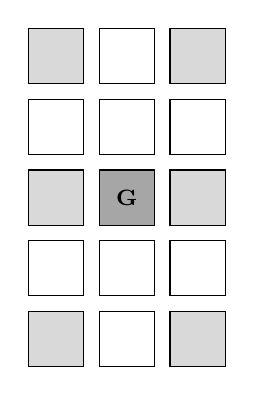
\begin{tikzpicture}[
      cell/.style={draw, minimum size=7mm, font=\footnotesize},
      wall/.style={cell, fill=black!15},
      free/.style={cell, fill=white},
      bottleneck/.style={cell, fill=black!35}
    ]
    \foreach \gx/\gy/\gkind in {0/0/wall,1/0/free,2/0/wall,0/1/free,1/1/free,2/1/free,0/2/wall,1/2/bottleneck,2/2/wall,0/3/free,1/3/free,2/3/free,0/4/wall,1/4/free,2/4/wall}{%
      \node[\gkind] at (\gx*0.9,-\gy*0.9) {};
    }
    \node[font=\footnotesize] at (1*0.9,-2*0.9) {\textbf{G}};
  \end{tikzpicture}
  \caption{Exemplo ilustrativo de gargalo estrutural: células cinza-claras
    são paredes, células brancas são caminho livre, e a célula cinza-escura
    marcada com ``G'' é o único ponto de passagem entre as duas metades do
    nível.}
  \Description{Grade de 5 linhas por 3 colunas representando um corredor.
  As colunas das extremidades alternam entre parede e caminho livre nas
  linhas superior e inferior, enquanto a coluna central possui uma única
  célula de passagem, destacada e marcada com a letra G, conectando as
  duas metades do nível.}
  \label{fig:exemplo-grid}
\end{figure}

Nesse exemplo, um agente de navegação ingênuo (por exemplo, treinado
apenas com recompensa esparsa por atingir a saída) tende a atravessar a
célula \textbf{G} com a mesma frequência que qualquer outra célula do
caminho, uma vez que ela é, por definição, o único caminho possível --
não há, portanto, sinal de que essa célula seja estruturalmente diferente
das demais apenas observando a frequência de visitação. É por isso que a
Equação~\eqref{eq:reward-ext} pondera o fluxo $\tau(v)$ pela centralidade
$w(v)$ da célula no grafo de navegação: a célula \textbf{G} possui
centralidade de intermediação (\emph{betweenness centrality}) muito mais
alta do que as demais células do corredor, pois todo caminho entre as duas
metades do nível necessariamente passa por ela. Um valor de $\tau(v)$
comparável ao das demais células livres, combinado com um peso $w(v)$
elevado, é o que sinaliza \textbf{G} como um gargalo estrutural relevante,
e não apenas mais uma célula de passagem. Em corredores com múltiplos
caminhos alternativos, por outro lado, a centralidade de cada célula
individual tende a ser menor, e um gargalo só emerge quando o fluxo
observado $\tau(v)$ cai significativamente abaixo do esperado para células
de centralidade comparável -- é essa combinação entre topologia estática
($w(v)$) e comportamento dinâmico observado ($\tau(v)$) que buscamos
capturar com a função de recompensa proposta, e que uma heurística
puramente estrutural (que considerasse apenas $w(v)$) não conseguiria
distinguir sozinha.

\section{Arquitetura do Sistema}
\label{sec:arquitetura}

A Figura~\ref{fig:pipeline} ilustra o pipeline proposto, do ambiente Godot
até a política de ação, passando pelos três componentes descritos a seguir.

\begin{figure}
  \centering
  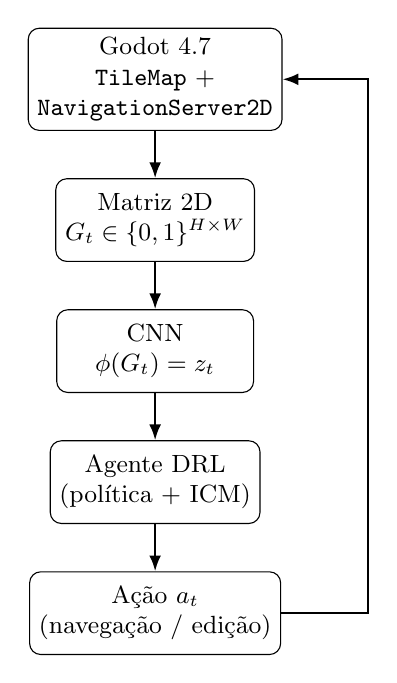
\begin{tikzpicture}[
      node distance=6mm,
      box/.style={draw, rounded corners, align=center, minimum height=1.05cm,
        minimum width=2.5cm, font=\small},
      arrow/.style={-{Latex[length=2mm]}, thick}
    ]
    \node[box] (godot) {Godot 4.7\\\texttt{TileMap} +\\\texttt{NavigationServer2D}};
    \node[box, below=of godot] (grid) {Matriz 2D\\$G_t \in \{0,1\}^{H\times W}$};
    \node[box, below=of grid] (cnn) {CNN\\$\phi(G_t) = z_t$};
    \node[box, below=of cnn] (drl) {Agente DRL\\(política + ICM)};
    \node[box, below=of drl] (action) {Ação $a_t$\\(navegação / edição)};
    \draw[arrow] (godot) -- (grid);
    \draw[arrow] (grid) -- (cnn);
    \draw[arrow] (cnn) -- (drl);
    \draw[arrow] (drl) -- (action);
    \draw[arrow] (action.east) -- ++(1.1,0) |- (godot.east);
  \end{tikzpicture}
  \caption{Pipeline proposto: extração da matriz do nível, processamento
    espacial via CNN, decisão do agente de DRL e retroalimentação da ação
    para o ambiente Godot.}
  \Description{Diagrama de fluxo vertical mostrando quatro etapas
    conectadas por setas: Godot com TileMap e NavigationServer2D produz uma
    matriz 2D; a matriz é processada por uma CNN, gerando um vetor latente;
    esse vetor alimenta o agente de aprendizado por reforço profundo, que
    produz uma ação; a ação retroalimenta o ambiente Godot, fechando o
    ciclo.}
  \label{fig:pipeline}
\end{figure}

\subsection{Ambiente de Desenvolvimento}

O ambiente de desenvolvimento está sendo estruturado na engine
Godot~4.7~\cite{godotengine}, escolhida por seu suporte nativo a física 2D
determinística, seu sistema de navegação (\texttt{NavigationServer2D}) e a
facilidade de introspecção de dados de cena via GDScript, o que permite
extrair a representação estruturada do nível sem a necessidade de
processamento de imagem.

\subsection{Representação do Ambiente}
\label{sec:representacao-ambiente}

Após avaliação da melhor estratégia de \emph{input} para a IA, descartou-se
o uso de imagens diretas da câmera (renderização de pixels): o
processamento de texturas e iluminação adicionaria um custo computacional
desnecessário à rede neural, sem agregar informação relevante para a tarefa
de identificação de gargalos, que é fundamentalmente estrutural, e não
visual.

A solução estabelecida é a extração estruturada do mapa na forma de uma
matriz 2D (\emph{grid}). Utilizando os recursos do Godot 4.7, mapeia-se o
\texttt{TileMap} e as malhas do \texttt{NavigationServer2D} para gerar um
\emph{array} bidimensional cujos valores representam os estados do
terreno:
\begin{itemize}
  \item \textbf{0}: caminho livre e navegável;
  \item \textbf{1}: parede ou obstáculo rígido.
\end{itemize}

Nesta etapa do projeto arquitetural, a geração dessa matriz limpa pelo
Godot foi isolada como uma ``caixa preta'' já funcional, permitindo
dedicação integral à modelagem da IA. A codificação binária inicial
($\{0,1\}$) foi escolhida por sua simplicidade; canais adicionais (posição
do agente, distância à saída, densidade histórica de tráfego) poderão ser
concatenados como planos extras da mesma matriz sem alterar a arquitetura
do extrator convolucional, apenas o número de canais de entrada.

\subsection{Processamento Espacial com Redes Convolucionais}
\label{sec:cnn}

A matriz 2D gerada atua como a observação (\emph{state}) para a rede
neural. Para extrair os padrões topológicos desse ambiente espacial ---
como corredores estreitos, rotas críticas e densidade de obstáculos --- os
dados passam por uma \emph{Deep Convolutional
Network}~\cite{lecun1998gradient} (CNN). A natureza das CNNs permite que o
modelo compreenda o nível de forma geométrica, em vez de apenas ler números
isolados, o que é essencial para reconhecer padrões espaciais que
caracterizam um gargalo.

O projeto atual do extrator segue o padrão consolidado por trabalhos de RL
sobre grades (\emph{grid-world}), com camadas convolucionais de
\emph{stride} $1$ e \emph{kernels} pequenos ($3\times3$), preservando a
granularidade de \emph{tile} necessária para localizar precisamente um
gargalo, seguidas de uma camada totalmente conectada que produz o vetor
latente $z_t \in \mathbb{R}^d$ utilizado pela política e pelo módulo de
curiosidade. Optamos por não utilizar operações de \emph{max-pooling}
agressivas, que tenderiam a borrar exatamente as estruturas finas
(corredores de largura igual a um \emph{tile}) que o sistema precisa
detectar.

\subsection{Agente de Deep Reinforcement Learning}

A tomada de decisão e a exploração do mapa utilizam uma arquitetura de
Aprendizado por Reforço Profundo. O modelo é construído com base em
conceitos avançados da literatura, unindo \emph{Curiosity-Driven
Exploration}~\cite{pathak2017curiosity} com as bases do
PCGRL~\cite{khalifa2020pcgrl}. A Tabela~\ref{tab:drl} resume os três
componentes centrais do sistema segundo a formalização apresentada na
Seção~\ref{sec:formalizacao}.

\begin{table}
  \caption{Componentes do sistema de Aprendizado por Reforço Profundo}
  \label{tab:drl}
  \begin{tabular}{p{0.28\linewidth}p{0.6\linewidth}}
    \toprule
    \textbf{Componente} & \textbf{Estratégia no projeto} \\
    \midrule
    Observação (\emph{State}) & A matriz 2D processada pela CNN,
      representando a topologia instantânea da fase ($z_t = \phi(G_t)$). \\
    Ação (\emph{Action}) & Navegação vetorial discreta e, posteriormente, a
      capacidade de sinalizar ou modificar tiles (adicionar/remover
      bloqueios). \\
    Recompensa (\emph{Reward}) & Combinação extrínseca/intrínseca: penaliza
      fortemente áreas de baixo fluxo de travessia (gargalos) e recompensa
      a exploração de regiões mal modeladas pelo agente. \\
    \bottomrule
  \end{tabular}
\end{table}

Quanto ao algoritmo de otimização de política, optamos por explorar
\emph{Proximal Policy Optimization}
(PPO)~\cite{schulman2017proximal}, em vez de métodos baseados em valor como
\emph{Deep Q-Networks}. Essa escolha se justifica por três razões: (i) o
espaço de ações proposto na Seção~\ref{sec:acao} é naturalmente discreto,
mas será estendido a variações contínuas de intensidade de edição em fases
futuras, e o PPO acomoda ambos os casos sem mudança estrutural; (ii) o PPO
é conhecido por sua estabilidade de treinamento em cenários com recompensas
esparsas e ruidosas -- exatamente o cenário esperado ao combinar os termos
extrínseco e intrínseco da Equação~\eqref{eq:reward}; e (iii) sua natureza
\emph{on-policy} simplifica a integração com o módulo de curiosidade, que
depende de trajetórias recentes e consistentes com a política atual para
que o erro de predição do modelo dinâmico seja informativo.

\subsection{Integração de Dados e Pipeline de Treinamento}

A integração entre o ambiente Godot e o ambiente de treinamento (Python)
está planejada por meio de um protocolo de comunicação por sockets locais,
no qual o Godot exporta, a cada \emph{step} de simulação, a matriz $G_t$
serializada e recebe de volta a ação $a_t$ escolhida pela política. Essa
separação de processos permite que o treinamento seja acelerado por
hardware dedicado (GPU) sem sobrecarregar o laço de renderização e física
do motor de jogo, e permite, no futuro, paralelizar múltiplas instâncias do
ambiente para acelerar a coleta de trajetórias, uma prática comum em
\emph{pipelines} de RL profundo.

\section{Estado Atual da Implementação}
\label{sec:estado}

Com a comunicação base e o escopo da IA (matriz 2D~$\rightarrow$~CNN~$
\rightarrow$~DRL) validados e definidos, o projeto avança para a
estruturação formal do aprendizado de máquina. Até o momento:
\begin{itemize}
  \item a extração da matriz 2D a partir do \texttt{TileMap} e do
    \texttt{NavigationServer2D} foi implementada e isolada como módulo
    independente, funcionando de forma estável para os níveis de teste
    utilizados durante o desenvolvimento;
  \item o desenho geral do pipeline \emph{CNN~+~DRL} (Seção~\ref{sec:arquitetura})
    foi definido e revisado frente à literatura de PCGRL e de exploração
    por curiosidade;
  \item a formalização do problema como MDP (Seção~\ref{sec:formalizacao}),
    incluindo a proposta inicial da função de recompensa híbrida, foi
    concluída nesta etapa do relatório; e
  \item o treinamento do agente ainda não foi iniciado -- os itens acima
    constituem a base arquitetural sobre a qual os experimentos descritos
    na Seção~\ref{sec:avaliacao} serão conduzidos.
\end{itemize}

\section{Metodologia de Avaliação Proposta}
\label{sec:avaliacao}

Como o treinamento do agente ainda está em fase de estruturação, esta
seção descreve a metodologia de avaliação planejada para os próximos
ciclos do projeto, e não resultados experimentais já obtidos.

\subsection{Métricas}

Propomos as seguintes métricas para avaliar a capacidade do agente de
identificar gargalos:
\begin{itemize}
  \item \textbf{Precisão de detecção}: fração das células sinalizadas pelo
    agente como gargalo que coincidem com gargalos identificados por
    especialistas humanos em um conjunto de níveis de referência anotados
    manualmente;
  \item \textbf{Cobertura (\emph{recall})}: fração dos gargalos anotados
    manualmente que são efetivamente sinalizados pelo agente;
  \item \textbf{Entropia do mapa de visitação}: dispersão espacial das
    trajetórias do agente ao longo de um episódio, utilizada como
    \emph{proxy} para verificar se a exploração guiada por curiosidade está
    de fato cobrindo regiões de baixo fluxo, e não apenas reforçando rotas
    já bem conhecidas; e
  \item \textbf{Redução de gargalos pós-edição}: para a fase futura de
    ações de edição (Seção~\ref{sec:acao}), a variação do fluxo de
    travessia $\tau(v)$ antes e depois das intervenções sugeridas pelo
    agente.
\end{itemize}

\subsection{Baselines}

Como referência de comparação, planejamos incluir:
\begin{itemize}
  \item um agente aleatório, que executa ações de navegação uniformemente
    ao acaso, para calibrar o piso de desempenho das métricas acima;
  \item um agente de \emph{pathfinding} clássico (busca A* sobre o grafo de
    navegação), que representa a linha de base ``sem aprendizado'' e
    permite isolar o ganho específico atribuível ao componente de DRL; e
  \item uma variante do próprio agente proposto sem o termo intrínseco de
    curiosidade ($\beta = 0$ na Equação~\eqref{eq:reward}), para medir a
    contribuição isolada da exploração guiada por curiosidade em relação à
    recompensa puramente extrínseca.
\end{itemize}

\subsection{Protocolo Experimental}

O protocolo planejado consiste em treinar cada configuração do agente em um
conjunto fixo de níveis de treinamento, avaliando periodicamente em um
conjunto de validação de níveis não vistos durante o treinamento, de forma a
verificar a generalização da política para topologias distintas das
utilizadas no treinamento -- um requisito essencial para que a ferramenta
seja útil em cenários reais de \emph{level design}, nos quais o agente deve
avaliar níveis inéditos, e não apenas os níveis sobre os quais foi treinado.
Cada configuração será executada com múltiplas sementes aleatórias para
permitir a análise de variância entre execuções, prática recomendada na
literatura de aprendizado por reforço~\cite{sutton2018reinforcement} dada a
sensibilidade conhecida desses métodos à inicialização e à ordem de
amostragem das trajetórias.

\section{Discussão: Limitações e Riscos}
\label{sec:discussao}

Ainda que a arquitetura proposta seja promissora, alguns riscos
metodológicos merecem discussão explícita nesta etapa do projeto.

\textbf{Risco de \emph{reward hacking}.} A combinação de recompensa
extrínseca e intrínseca (Equação~\eqref{eq:reward}) introduz o risco
clássico de que o agente explore artefatos da própria função de recompensa
em vez de resolver o problema pretendido -- por exemplo, permanecer em
regiões cujo modelo dinâmico é intencionalmente difícil de prever (como
áreas com física caótica), gerando recompensa intrínseca alta sem
corresponder a um gargalo real de \emph{design}. Mitigar esse risco exigirá
normalização cuidadosa do termo $r^{\text{int}}_t$ e, possivelmente, seu
decaimento ao longo do treinamento, à medida que o modelo dinâmico se torna
mais preciso.

\textbf{Generalização entre temas visuais e topológicos.} Como a
representação de estado é puramente estrutural (matriz binária), espera-se
melhor generalização entre temas visuais distintos do que abordagens
baseadas em pixels; entretanto, a generalização entre topologias
estruturalmente muito diferentes das vistas em treinamento (por exemplo,
níveis com geometria não ortogonal) ainda não foi avaliada e é um risco em
aberto.

\textbf{Custo computacional do treinamento distribuído.} A separação entre
o processo do Godot e o processo de treinamento (Seção~\ref{sec:arquitetura})
introduz sobrecarga de comunicação que pode se tornar um gargalo de
desempenho -- de forma irônica, o próprio pipeline de treinamento pode sofrer
do tipo de problema que o agente é treinado para detectar no nível do jogo.
Essa sobrecarga precisará ser medida empiricamente antes de escalar o
número de ambientes paralelos.

\textbf{Validação com especialistas humanos.} As métricas de precisão e
cobertura propostas na Seção~\ref{sec:avaliacao} dependem da anotação manual
de gargalos por especialistas, um processo que introduz subjetividade e que
ainda precisa ser operacionalizado -- por exemplo, definindo um protocolo de
anotação com múltiplos anotadores e medidas de concordância entre eles.

\section{Considerações Éticas e de Uso Responsável}
\label{sec:etica}

Ferramentas de diagnóstico automatizado de \emph{level design} levantam
questões de uso responsável que merecem consideração explícita, mesmo em
uma etapa inicial do projeto como a aqui relatada.

\textbf{Complementaridade, não substituição, do julgamento humano.} O
sistema proposto tem como objetivo fornecer um sinal quantitativo adicional
ao processo de \emph{design}, e não substituir o julgamento de designers
humanos sobre o que torna um nível interessante. Um gargalo identificado
pelo agente pode ser, em certos contextos de \emph{design} intencional
(por exemplo, um estrangulamento tático em um mapa competitivo), uma
característica desejada, e não um defeito a ser corrigido. A ferramenta
deve, portanto, ser utilizada como apoio à decisão, com a palavra final
permanecendo com a equipe de \emph{design}.

\textbf{Viés na definição de fluidez.} A métrica de fluxo de travessia
$\tau(v)$ e os pesos $w(v)$ de centralidade (Seção~\ref{sec:recompensa})
embutem uma definição específica -- e necessariamente parcial -- do que
constitui um nível ``fluido''. Essa definição pode não ser representativa
de todos os estilos de jogo ou de todos os perfis de jogadores (por
exemplo, jogadores que preferem exploração lenta a progressão rápida), e
deve ser comunicada de forma transparente a quem utilizar a ferramenta,
para evitar que recomendações automatizadas sejam interpretadas como
verdades objetivas sobre qualidade de \emph{design}.

\textbf{Dados de jogadores reais.} Na fase atual do projeto, todo o
treinamento ocorre em simulação, sem coleta de dados de jogadores humanos.
Caso etapas futuras incorporem dados de \emph{playtesting} real -- por
exemplo, para calibrar $\tau(v)$ com telemetria de partidas humanas --
será necessário um protocolo explícito de consentimento e anonimização,
seguindo as práticas usuais de pesquisa com participantes humanos.

\section{Trabalhos Futuros}
\label{sec:futuro}

Com a arquitetura e a formalização do problema definidas, os próximos
passos do projeto incluem:
\begin{enumerate}
  \item \textbf{Implementação da função de recompensa:} implementar e
    calibrar experimentalmente os pesos $\beta$, $\eta$ e $\theta_\tau$ das
    Equações~\eqref{eq:reward}--\eqref{eq:reward-int}, hoje definidos apenas
    em nível conceitual;
  \item \textbf{Implementação do espaço de ações de edição:} estender o
    espaço de ações de navegação para incluir as ações de sinalização e
    edição de tiles descritas na Seção~\ref{sec:acao};
  \item \textbf{Integração de dados:} implementar o protocolo de
    comunicação por sockets entre o Godot e o ambiente de treinamento
    descrito na Seção~\ref{sec:arquitetura};
  \item \textbf{Construção do conjunto de níveis de referência:} preparar o
    conjunto de níveis anotados manualmente necessário para as métricas de
    precisão e cobertura da Seção~\ref{sec:avaliacao};
  \item \textbf{Execução dos experimentos-piloto:} treinar as primeiras
    versões do agente e dos \emph{baselines} propostos, permitindo uma
    primeira validação empírica -- ainda que preliminar -- da arquitetura
    descrita neste artigo; e
  \item \textbf{Extensão para mecânicas multiplayer:} avaliar como o fluxo
    de travessia $\tau(v)$ deve ser redefinido quando múltiplos agentes
    ocupam o mesmo nível simultaneamente, disputando o mesmo espaço físico.
\end{enumerate}

\section{Conclusão}
\label{sec:conclusao}

Este artigo relatou o andamento e a arquitetura em desenvolvimento de um
agente de Aprendizado por Reforço Profundo para identificação e correção de
gargalos de \emph{level design} em jogos 2D construídos na engine Godot. A
representação do ambiente como matriz 2D, processada por uma CNN e
consumida por um agente de DRL inspirado em PCGRL e em exploração guiada
por curiosidade, oferece um caminho concreto para ir além do
\emph{pathfinding} tradicional. Formalizamos o problema como um Processo de
Decisão de Markov, propusemos uma função de recompensa híbrida
extrínseca/intrínseca e delineamos uma metodologia de avaliação -- com
métricas, \emph{baselines} e protocolo experimental -- para os próximos
ciclos do projeto. Discutimos também os riscos metodológicos mais
relevantes, em particular o risco de \emph{reward hacking} inerente ao uso
de recompensas intrínsecas. Os trabalhos futuros mais imediatos --
implementação da função de recompensa, do espaço de ações de edição e da
integração de dados -- consolidarão a base necessária para os primeiros
experimentos-piloto de treinamento do agente.

\begin{acks}
Agradecemos ao Prof.\ Augusto Baffa pela orientação ao longo do
desenvolvimento deste projeto, no âmbito da disciplina Projeto Orientado IV
(INF1824) da PUC-Rio.
\end{acks}

\label{fim-conteudo}
\bibliographystyle{ACM-Reference-Format}
\bibliography{references}

\end{document}
